% Slides for 2025-07-01
% To create a slide, use the following:
% \begin{frame}{TITLE}
%     BODY
% \end{frame}

% To create a slide with a bullet list, use the following:
% \begin{frame}{TITLE}
%     \begin{itemize}
%         \item ITEM 1
%         \item ITEM 2
%     \end{itemize}    
% \end{frame}

% To create a slide with numbered list, use the following:
% \begin{frame}{TITLE}
%     \begin{enumerate}
%         \item ITEM 1
%         \item ITEM 2
%     \end{enumerate}
% \end{frame}

% To create a slide with a graphic:
% 1. Add the graphic to this folder (named picture.png)
% 2. Use the following:
% \begin{frame}{TITLE}
%     \centering
%     \includegraphics[height=0.7\textheight,width=0.7\textwidth,keepaspectratio]{picture.png}
% \end{frame}

% To create a slide with two columns, use the following:
% \begin{frame}{TITLE}
%     \begin{columns}
%         \begin{column}{0.5\textwidth}
%             COLUMN 1 BODY
%         \end{column}
%         \begin{column}{0.5\textwidth}
%             COLUMN 2 BODY
%         \end{column}
%     \end{columns}
% \end{frame}

%Introduction 
\begin{frame}{HallPass}
    \begin{columns}
        \begin{column}{0.5\textwidth}
            \begin{itemize}
                \item Controller: Processors, DMA etc.
                \item Interconnect: Arbitrates access
                \item Peripherals: Memory, I/O devices
            \end{itemize} 
        \end{column}
        \begin{column}{0.5\textwidth}
            \begin{figure}
                \centering
                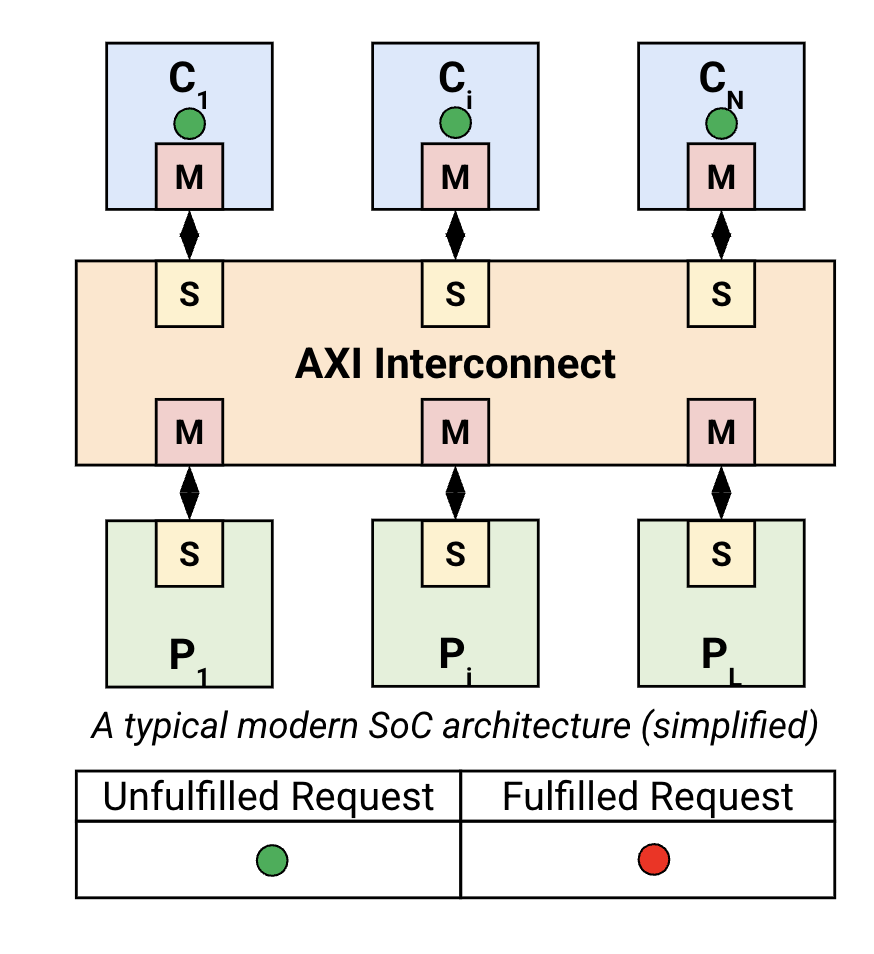
\includegraphics[height=0.7\textheight,width=0.7\textwidth,keepaspectratio]{SoC.png}
                \caption{System on Chip (SoC)}
            \end{figure}
            \end{column}
    \end{columns}
\end{frame}

%Background
\begin{frame}{HallPass-Background}
    \begin{columns}
        \begin{column}{0.5\textwidth}
            AKER Access Control System
            \begin{itemize}
                \item Access Control Wrappers (ACWs)
            \end{itemize}
        \end{column}
        \begin{column}{0.5\textwidth}
            \begin{figure}
            \centering
            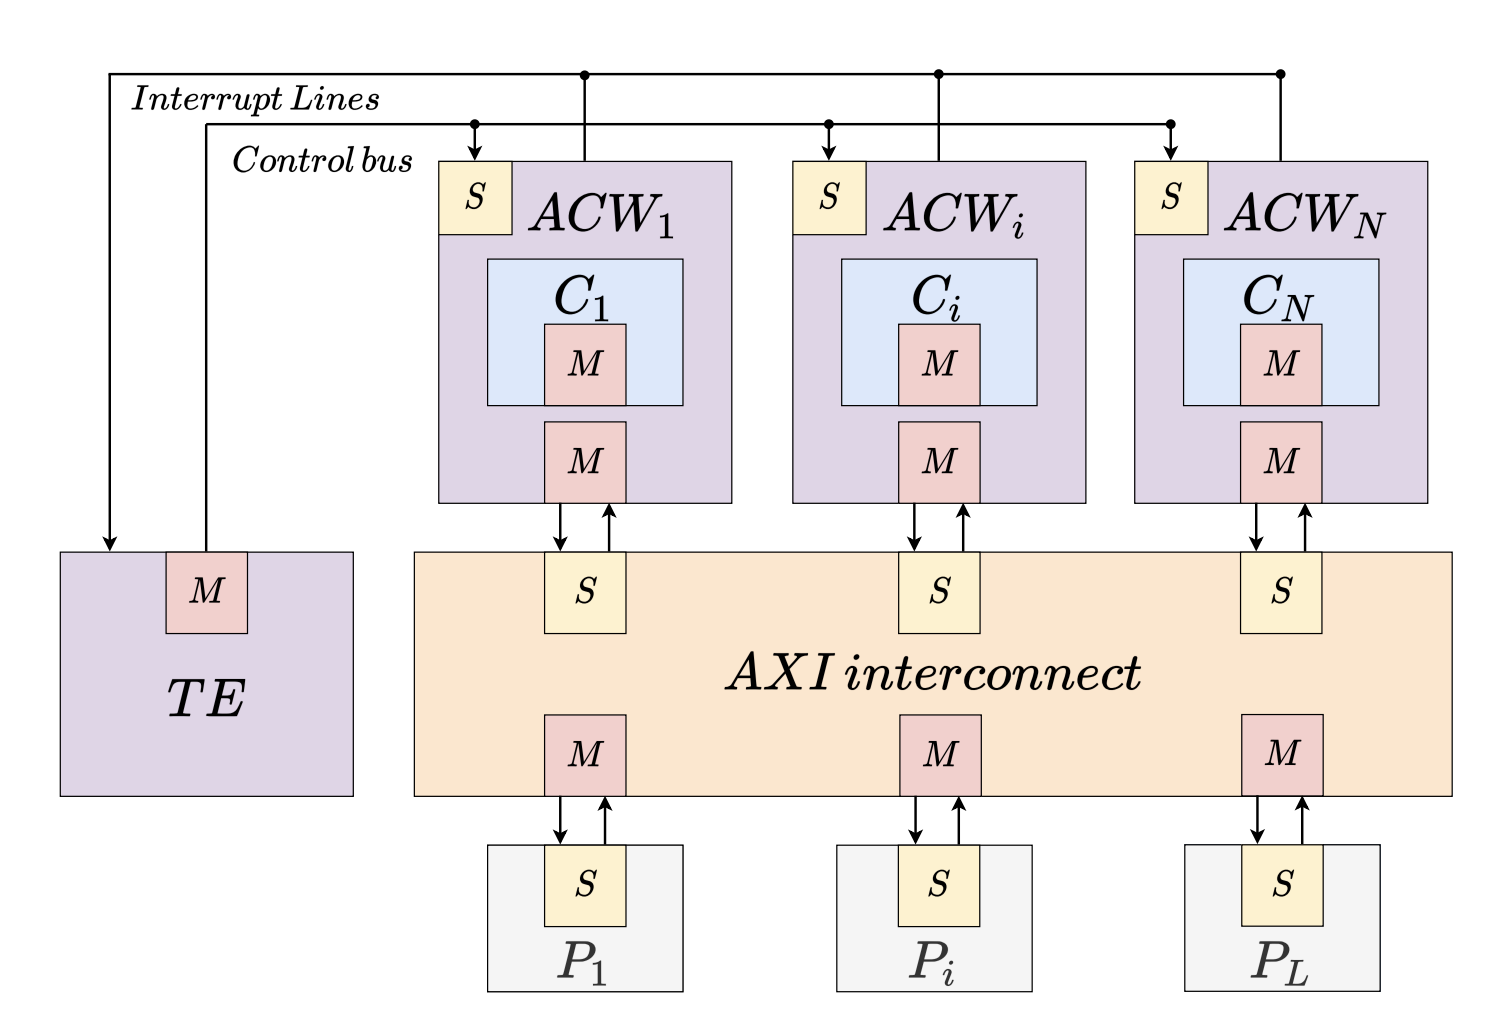
\includegraphics[height=0.7\textheight,width=0.7\textwidth,keepaspectratio]{aker.png}
            \caption{AKER Access Control System}
            \end{figure}
        \end{column}
    \end{columns}
\end{frame}

%Problem
\begin{frame}{HallPass-Problem}
    \begin{columns}
        \begin{column}{0.5\textwidth}
            Unintended Proxy
        \end{column}
        \begin{column}{0.5\textwidth}
            \begin{figure}
            \centering
            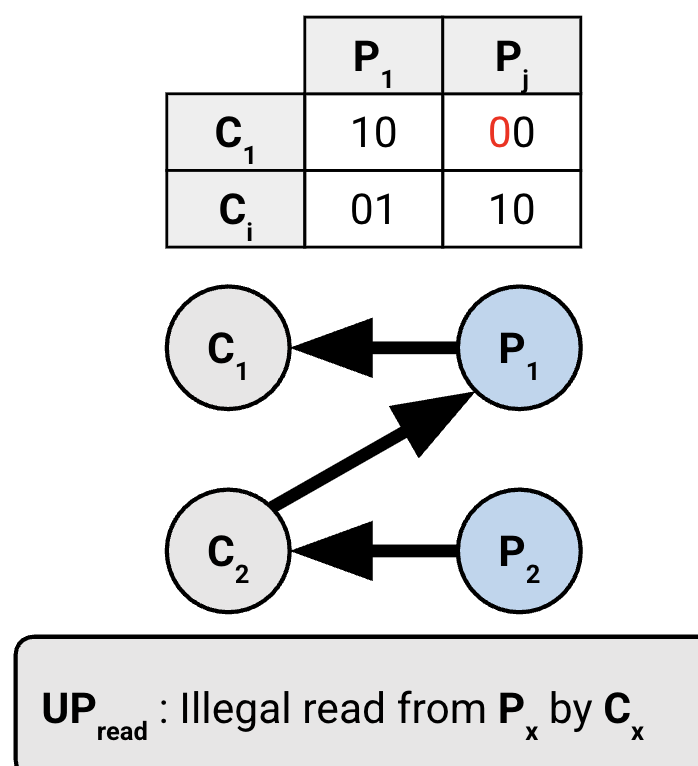
\includegraphics[height=0.7\textheight,width=0.7\textwidth,keepaspectratio]{proxy.png}
            \caption{Unintended Proxy}
        \end{figure}
        \end{column}
    \end{columns}
\end{frame}

%Solution
\begin{frame}{HallPass-Solution}
    \begin{columns}
        \begin{column}{0.5\textwidth}
        Power Performance Area (PPA) Tradeoffs
        \end{column}
        \begin{column}{0.5\textwidth}
            \begin{figure}
            \centering
            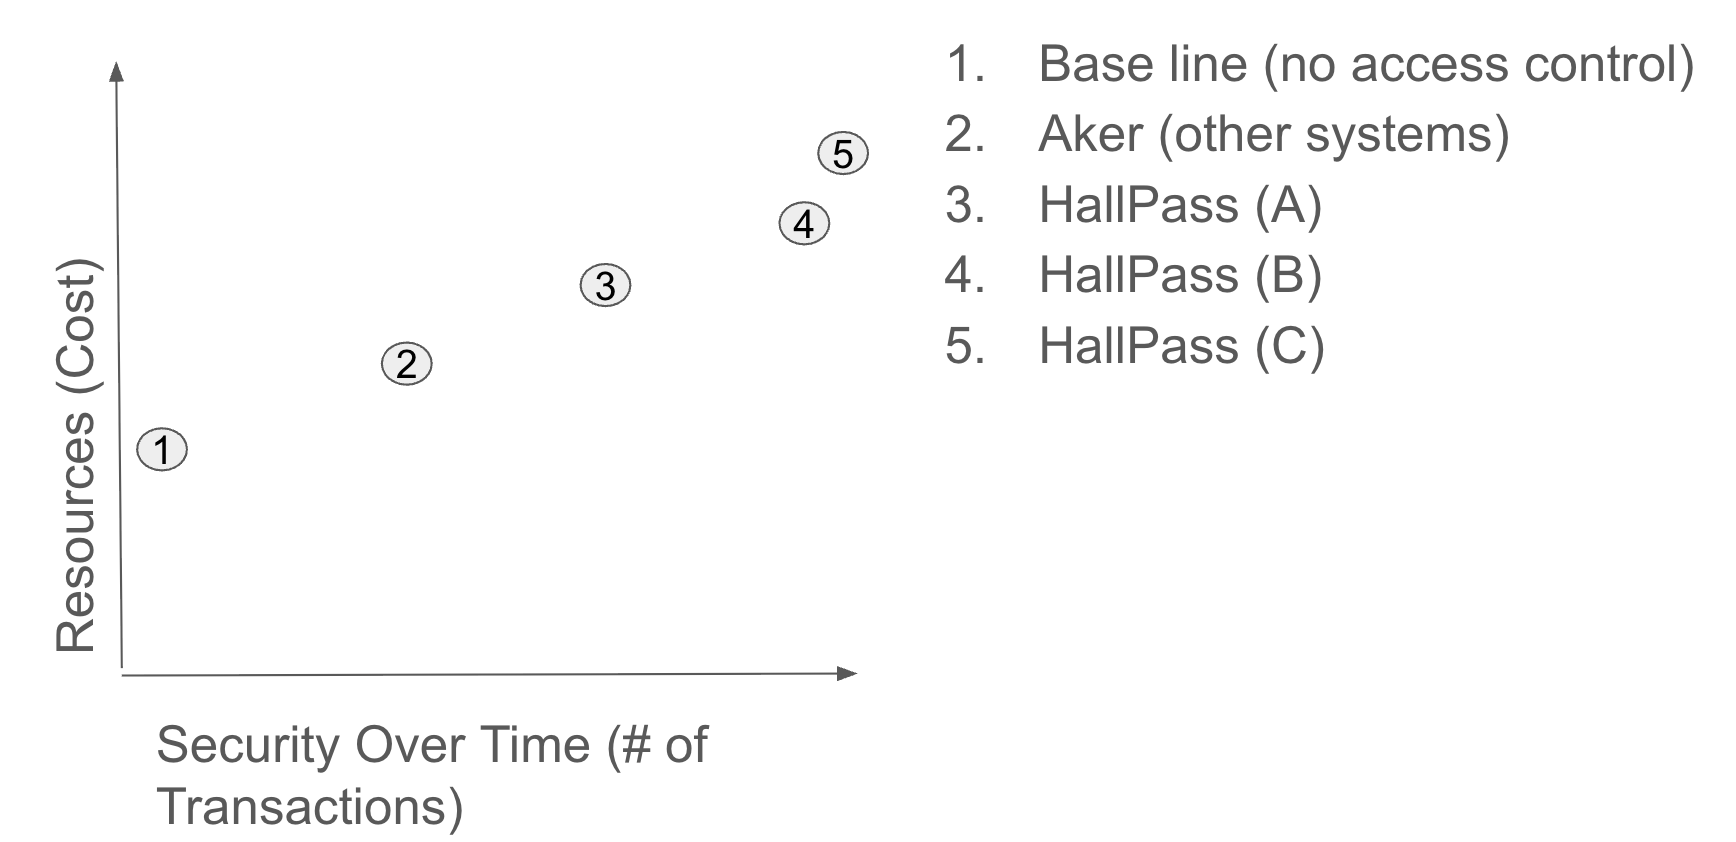
\includegraphics[height=0.7\textheight,width=0.7\textwidth,keepaspectratio]{tradeoffs.png}
            \caption{PPA Tradeoffs}
            \end{figure}
        \end{column}
    \end{columns}
\end{frame}
